%\vspace{-5pt}
\section{Conclusions and Future Work}
\label{sec:conclusions}

We found that a learning based approach extracts some interesting patterns,
that cannot be captured by language rules.
We model tokens using dense word vectors and use natural language processing
methods such as 
a simple matrix-vector model, feed forward neural network models,
attention models and recurrent models.
These models do not use any information about the language grammar or syntax.
The attention based model performs the best, because it directly connects each
input token to output, and also computes weights for important tokens. It is
the most general of all models, with the most parameters.
We found that by adjusting the vector dimensions and number of layers, we could
reduce overfitting, and get close accuracies for training and test data.
Our top 3 predicted tokens give an accuracy of over 80\% for the cases where
the next token is known (a key or a postitional token), for Linux,
and over 60\% for Twisted.
A study of these vectors reveals a signficiant clustering of related tokens.

Though we did not use any information about language grammar and syntax, it
would be interesting to combine language rules with our learning based
approach. For example, we could prune our predictions to those that are only
syntactically valid. We could also increase our window size, and jointly
process \texttt{.h} and \texttt{.c} files, to improve the context. Such large
contexts may not scale well with feed-forward model, but recurrent models are
known to perform well with large inputs. We could also try to use language
rules to list out all possible options for next token, and then chain that to a
learning based model to improve the predictions. We could also try to learn
these language rules instead of listing them, by processing a large number of
different projects.

\begin{figure}
  \centering
\begin{subfigure}{\linewidth}
  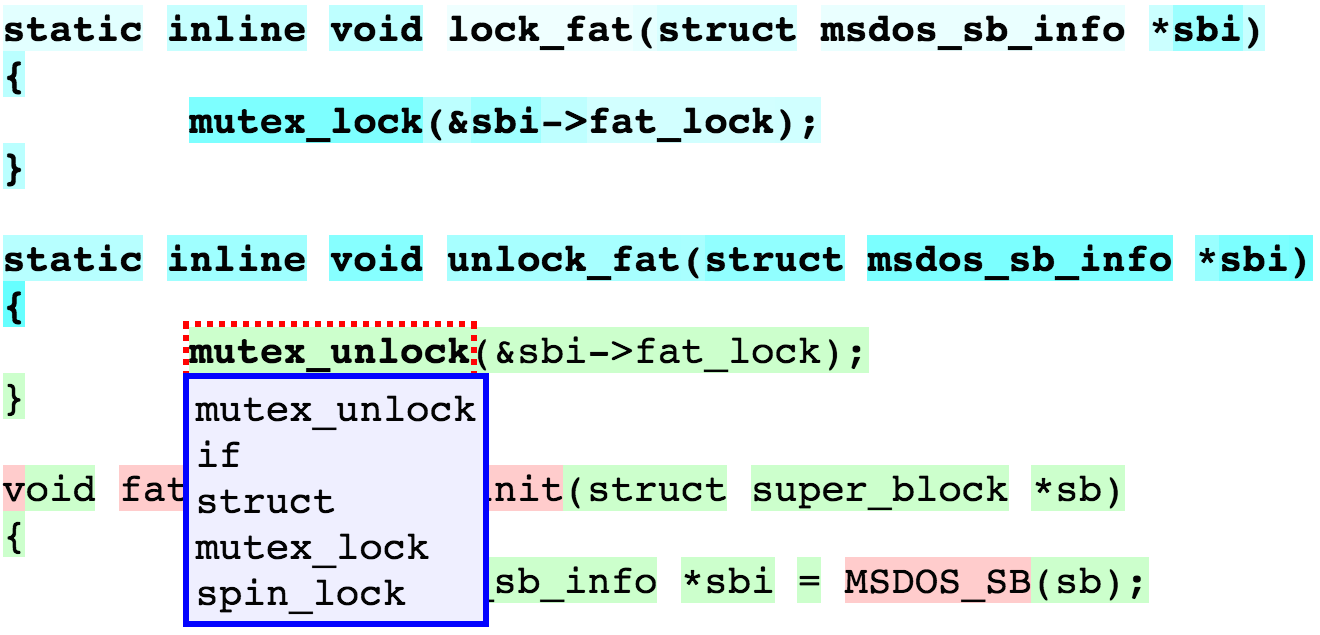
\includegraphics[width=\linewidth]{figs/example10.png}
  \caption{{\tt mutex\_lock} and {\tt mutex\_unlock} pair on same lock variable}
  \label{fig:lockunlock}
\end{subfigure}
\begin{subfigure}{\linewidth}
  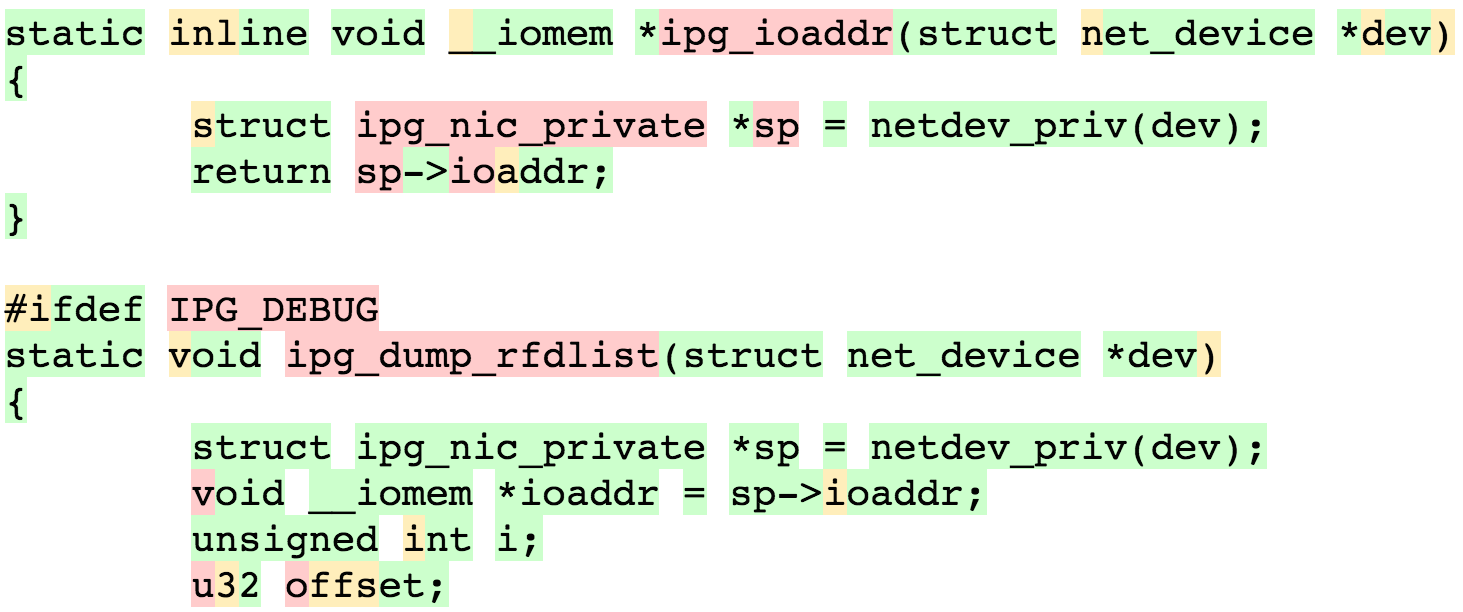
\includegraphics[width=\linewidth]{figs/example4.png}
  \caption{Duplicate code after function definition predicted correctly}
  \label{fig:duplicate}
\end{subfigure}
\begin{subfigure}{\linewidth}
  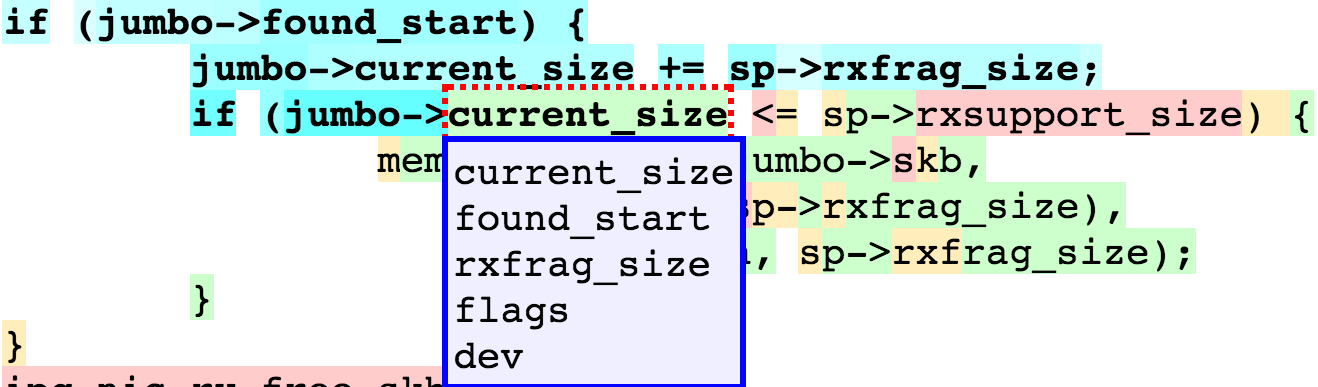
\includegraphics[width=\linewidth]{figs/example7.png}
  \caption{Member variables predicted correctly}
  \label{fig:memvar}
\end{subfigure}
\begin{subfigure}{\linewidth}
  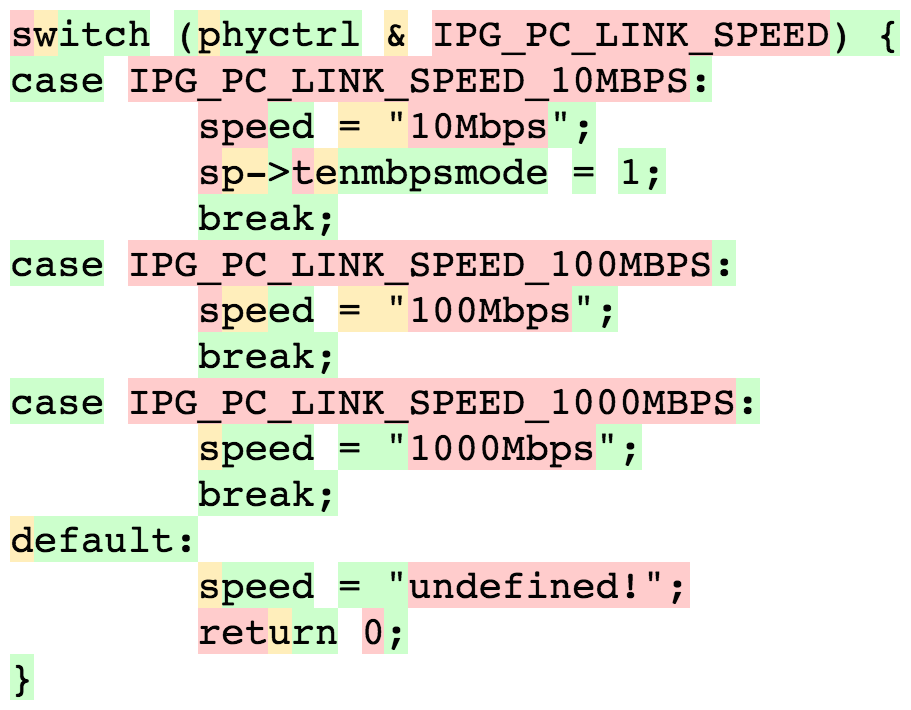
\includegraphics[width=0.6\linewidth]{figs/example1.png}
  \caption{{\tt case} token predicted correctly after each {\tt break;}}
  \label{fig:breakcase}
\end{subfigure}
  \caption{Interesting code patterns predicted correctly}
  \label{fig:ifpattern}
\end{figure}
